\documentclass{mscLiterature}
%
%
% Thesis data
%\mscDepartment{Delft Center for Systems and Control (\textsmaller{DCSC})}%
\mscProgram{Systems and Control}
%Change if needed to
%\mscProgram{Mechanical Engineering}
\mscFaculty{Mechanical, Maritime and Materials Engineering (3mE)}%
\mscName{Herminarto Nugroho}%
\mscDate{\today}%
\mscTitle{Deep Learning Neural Network for Tuning of the Optical Beamforming Networks}%
%\mscSubTitle{Optional Subtitle}%
\mscKeyWords{thesis, msc, subject}% only used in PDF properties
%\mscCoverPicture{STYLESTUFF/COVER}% to place a picture ( here the example COVER.eps) on the back of the cover page
%
\usepackage[numbers]{natbib}
\usepackage{amsmath}
% Third party options (create text/logo on the copywrite page)
%\mscThirdPartyText{The work in this thesis was supported by Aquaduct Swimming Supplies Incorporated. Their cooperation is hereby gratefully acknowledged.}
%\mscThirdPartyLogo{STYLESTUFF/EXAMPLELOGO}
% NOTE: on the title page only the TU Delft logo is permitted.
%
%
%
% Finalize the thesis data
\setThesisInfo
%
% Use \includeonly{} to build only certain parts of your thesis
%\includeonly{introduction, real_chapter, empty_chapter, long_chapter}%
%
%PH Toegevoegd 24-10-2011
%allow (matlab) listing max 1pt flexibility between lines
%\lstset{lineskip=0pt plus 1pt minus 0pt}
%
\begin{document}
%
%========================== Front matter ======================================
\frontmatter %
%
% Make the cover page and hell of a lot of title pages
\maketitle
%
%
% Abstract (does not appear in the Table of Contents)
\chapter*{Abstract}%

In an aircraft-satellite communications, the aircrafts transmit highly focused beams that are steered exactly towards the satellites. Conventional solution for this problem is to steer the dish antennas mechanically in order to direct the beam. Optical Beamforming Networks (OBFNs) instead, rely on many small and flat antennas that are coordinated in order to generate highly focused beams. In this project, a new type of OBFN proposed by \citet{Meijerink1} will be considered. The correct tuning of these OBFNs such that the beam is steered correctly is a difficult nonlinear problem that, so far, has only been addressed with off-the-shelf solvers in very small setups.

The problem of tuning a large-scale OBFN is very similar to training a neural network. For the later problem, many recent advances have been made under the umbrella term deep learning. The objective of this graduation project is to explore if and how advances in deep learning can be exploited to train the OBFNs. This can be achieved either by formulating the tuning problem as a learning problem, or by modifying existing algorithms in the area of deep learning. The tuning methodology developed in this project is based on feedback that can be measured in real systems (e.g., output power).

The literature survey is divided into two distinct parts. In the first part, we analyze the current setup and algorithm of OBFN proposed by \citet{Blokpoel} and \citet{Meijerink1} with special emphasis on the power optimality criterion. The analysis covers a whole concept of Antenna System, including Antenna Elements (AEs), OBFN based on binary tree topology, Optical Ring Resonators (ORRs), as well as the ORR's parameters and their influence to the group delay of the signal. The second part uses the theoretical information from the first part to support the implementation of deep learning neural network for solving a more general setup of OBFN without any limitation to small setups. This part handles the implementation of the concept of deep learning neural network to train the tuning of the OBFN.

It is expected that ....
(advantages of using neural network concept rather than current concept)


%
% table of contents, (\toc of \toclof of \tocloflot )
\tocloflot
%
%
%
% Preface
\chapter{Preface}

This is document is a part of my Master of Science graduation thesis. The idea of doing my thesis on this subject came after my scholarship committee, The Ministry of Communication and Information of the Republic of Indonesia required me to do research on the communication field. I remembered, Prof. dr. ir. Michel Verhaegen once presented some projects of his current research, and one of them is the project of control of airplane communication. I, later, contacted him asked about this project, and he then introduced me to my thesis supervisor, Dr. Sander Wahls whose expertise in communication.

The most important technical acknowledgment is made to Dr. Sander Wahls, for providing me with guidance and opportunities for learning telecommunication, a field which I am interested to yet not experienced in. I would also like to thank Laurens Bliek for his constant support and willingness to discuss the problems I have encountered in this project.

Moreover, I would like to thank all my friends with whom I traveled, shared incredible memories, laughter and joy. Finally, I would like to deeply thank my family who have supported me in all my endeavours and motivated me to aim higher.

An additional technical note is required: if any typo or incorrect information is detected please contact me via \verb|herminarto.nugroho@gmail.com| 


%%
% Acknowledgements
\chapter{Acknowledgements}%

I would like to thank my supervisor \mscreaderone\ for his assistance during the writing of this thesis\ldots

By the way, it might make sense to combine the Preface and the Acknowledgements.  This is just a matter of taste, of course.

\vspace*{15mm}

Delft, University of Technology \hfill \mscname \\
\mscdate
%%
% Dedication page. 
\cleardoublepage
\thispagestyle{empty}
\vspace*{\stretch{1}}

% Put your own motto here, or dedicate your work to your Mom or whatever...
\begin{quote}
\noindent``In the future, airplanes will be flown by a dog and a pilot. And the dog's job will be to make sure that if the pilot tries to touch any of the buttons, the dog bites him.''
	
--- \emph{Scott Adams}
\end{quote}

\vspace{\stretch{3}}
\clearemptydoublepage
%
%========================== Main matter ======================================
\mainmatter
%
%
% Introduction
\chapter{Introduction} \label{chap::intro}

Optical group delays are of great importance nowadays in optically-controlled \ac{PAA} system. \ac{PAA} system offers several advantages when compared to mechanically steered antennas, such as agile beam steering, relatively low maintenance cost, reduce drag force when applied in for instance vehicle and aircraft, and the possibility of supporting multiple antenna beams \citep{hansen2009phased}.

A \ac{PAA} system consists of an array of multiple \ac{AE}, corresponding transmission and/or reception units, and a beamformer. \ac{AE} signal consist of a time-delayed version of some desired signals, possible time-delayed version of of some undesired signals (from different direction), and noise (sky noise and antenna noise). The values of these delays are different for each \ac{AE}, depends on the geometrical distribution of the \ac{AE} locations, and for sure the direction of the incoming/outcoming wave-front signals. The beamformer consists of a delay-and-combine network that equalizes the delay values of the desired signal, such that the desired signal adds up in phase and reinforced, whereas the undesired signal do not add up and hence suppressed \citep{Meijerink1}. It is desirable that the time-delays are tunable, in order to be able to alter the reception angle of the \ac{PAA}. 

In this thesis, a seamlessly tunable optical beamformer concept proposed by \citet{meijerink2006phased} is used. It is based on coherent optical combining in an \ac{OBFN} using cascades of \ac{ORR} \citep{lenz2001optical,zhuang2005continuously} as tunable delay elements. With the structural enhancement (resonance) characteristic, the \ac{ORR} filters are able to generate a tunable group delay, which could be larger than the unit delay of the filter (the roundtrip time of the light). Thermal tuning mechanism is used in the filter, which is characterized by the high accuracy in the tuning process \citep{zhuang2005time}.

A \ac{NLP} optimization is one of the methods used to determine the parameters of the \ac{ORR} thermal tuning mechanism. This method converts a desired delay value into a set of optimal parameters of the respective \ac{ORR}. The first step of this method is to derive the optimality criteria. There are three optimality criteria, which are delay, phase and power criterion. From that three algorithms, an \ac{NLP} solver is used to find the optimal solution. This method was proposed by \citet{Blokpoel}. However, that method uses normalized bandwidths and target delays, and assumed the group delay response to be symmetric which shows its lack of generality. It is not desirable since it will limit the application of the one particular setting for the general case. Therefore, a more general method is proposed.

((((introduction about deep learning neural networks as an alternative solution))))

Taking the aforementioned premises into consideration, the goal of the thesis can now be
presented.

\section{Goals of the Thesis}
The main goal of the thesis is to provide a general method and algorithm for tuning the \ac{OBFN}, yielding better result without limitation on any binary tree \ac{OBFN} topology. This method will solve the basic problem the current tuning method (Non-linear Programming Optimization) has, which is designed to tune the \ac{OBFN} for a specific topology. This boils down to answer one question which is the fundamental
problem of this thesis:

\textit{``Is there a method that allows us to tune the OBFN for a general (in terms of topology and algorithm) and thus outperform the current Non-linear programming optimization method?''}


\section{Research Approach}

Based on the main goal of the thesis, the research approach can be divided into two parts containing several topics that must be addressed.

(((((topics to be addressed)))))

\section{Nomenclature}

Row or column vectors are represented using boldface lower-case symbols such as $\textbf{x}$. Boldface and upper-case symbols, such as $\textbf{A}$, are used for matrices. Regular font, $x_1$, denotes a scalar variable.

(((((edit every time needed)))))


%
% A Real Chapter
\chapter{Phased Array Antenna and Optical Ring Resonator: An Overview}

In the last century, radio systems have become an essential way to pass on signals by means of the transmission of electromagnetic waves with frequency below the visible light. In the recent years, increasing demand for fast information exchange motivated the development of many ideas of broadband radio applications. People wish to be able to connect to internet, participate in teleconference, or watch live TV no matter where they are, especially when traveling on a long intercontinental flight. This demand motivated the development of communication between satellite and aeroplanes.

In the application of the radio described above, the system is featured by the radio link with low signal power density. therefore, high-gain and direction-sensitive antennas are essentially required for the signal reception. The ordinary omni-directional antenna is not preferable because, although it is an directional-sensitive antenna, it has low gain \citep{cheng1989field}.

A conventional solution for a direction-sensitive antenna is a dish antenna, which can be steered mechanically to the point its main beam to a desired directions \citep{wilson2013tools}. Even though it is direction-sensitive and has high-gain, a dish antenna is slow because its speed is limited by the mechanical movement. The mechanical movement also have negative effect on the tuning precision. Another drawbacks are its large weight, large size, and aerodynamic drag effect when mounted on top of a plane. It also has difficulty for the maintenance. Instead of using a dish antenna, the more advantageous alternative is to use a \ac{PAA} \cite{balanis2008modern,MeijerinkPhased}. The explanation of \ac{PAA} will be covered in the first section of this chapter.

\section{Phased Array Antenna}
A \ac{PAA} consists of an array of \ac{AE}. The antenna pattern is determined by the geometry of the array as well as the signal amplitude and phase relation between the \ac{AE}s. The main beam of the \ac{PAA} can be steered without any mechanical movement involved. It is possible by changing the amplitude and the phase relation of the \ac{AE} signals. To control both the amplitudes and phases of the AE signals, the so-called beamformer is required. Conventionally a beamformer is realized in
the electrical domain. However, it can also be realized in the optical domain: an photonic beamformer. Compared to its
electrical counterpart, the photonic beamformer has the advantages, such as compactness, light weight, low loss, frequency independence, large instantaneous bandwidth, and inherent immunity to electromagnetic interference \citep{zhuang2010ring}. This fact makes the PAA comprising photonic beam former can be a preferable solution for the communication between satellite and aeroplanes.

The goal of beamformer is that the effective radiation pattern of the array is intensified in a desired direction and suppressed in undesired directions \citep{cheng1989field,balanis2008modern}. Then, the intensification of the radiation pattern in the desired direction results in the main beam of the array. The direction of the main beam can be steered by properly changing the phase relation between the AE signals. The illustration of the changing direction of the main beam is shown on the \figref{fig:beamformer_illustration}:

\begin{figure}[h]
	\centering
	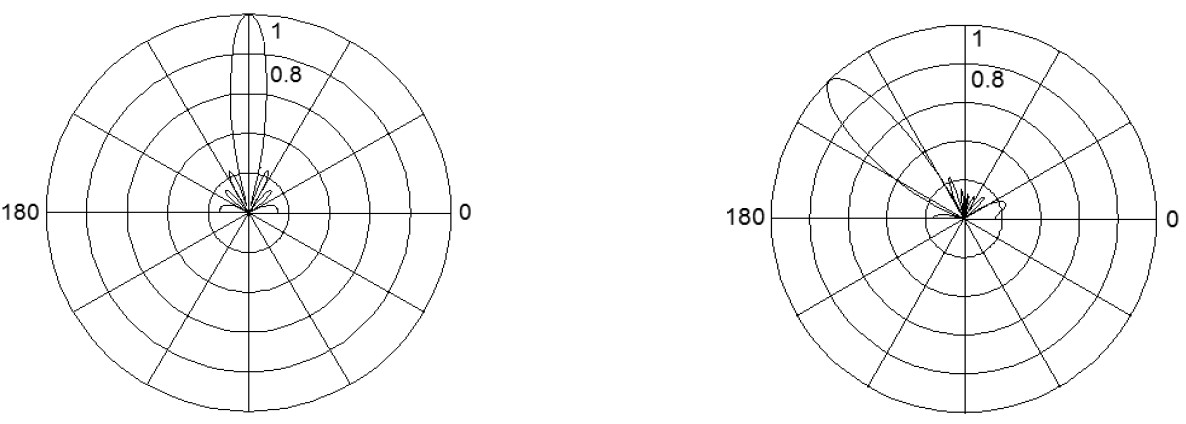
\includegraphics[width=0.8\textwidth]{images/beamformer_illustration}
	\caption{Illustration of (left) the main beam of an effective radiation pattern and (right) the beam steering effect. Source: \citep{zhuang2010ring}}
	\label{fig:beamformer_illustration}
\end{figure}

The simplest PAA is one-dimensional linear array antenna, which is based on gemetry of multiple identical AEs equally spaced along a single line. Although there are various array geometries as explained in \citep{cheng1989field,balanis2008modern}, to understand the basic principle of PAA, the one-dimensional linear array antenna is sufficient. \figref{fig:linear_array_antenna} shows the illustration of a simple 4-element linear array antenna.

\begin{figure}[h]
	\centering
	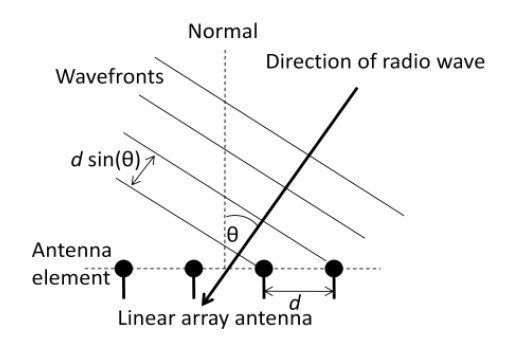
\includegraphics[width=0.5\textwidth]{images/linear_array_antenna}
	\caption{Illustration of a 4-element one-dimensional linear array antenna. Source: \citep{zhuang2010ring}}
	\label{fig:linear_array_antenna}
\end{figure}

Suppose the direction of the radio wave is coming at an angle of $\theta$ with respect to perpendicular direction of the surface of the PAA (called normal direction). Then all the spatial points have the same phase form a wavefront which is perpendicular to propagation direction of the wave, and this wavefront will reach each AE at a different time instance. The formula for the difference of the time arrival of the neighboring AE is given as:

\begin{equation}\label{eq:time_delay}
	\Delta t_a(d,\theta)=\frac{d \sin(\theta)}{c_0}
\end{equation}
where $d$ is the spacing between the AEs and $c_0$ is the speed of light in vacuum. This results in an interelement phase difference:

\begin{equation}\label{eq:phase_diff}
	\Delta \varphi (d,\theta,f)=2\pi f \Delta t_a(d,\theta)
\end{equation}
where $f$ is the frequency of the \ac{RF} wave.

When this interelement phase difference $\Delta \varphi (d,\theta,f)$ is removed by the additional phase compensation between two neighboring AEs $\Delta \delta = -\Delta \varphi (d,\theta,f)$ , the signals from different AEs will be in
phase and can be combined coherently. Then after combining the signals the intensification will be achieved for this particular receiving angle $\theta$. The signals coming from a different angle $\theta '$ will result in $\Delta \varphi (d,\theta ',f)$ which will not be cancelled out by $\Delta \delta$. Then due to the remaining phase difference between the AEs,
suppression of the signal will occur after the signal combining of the array. Furthermore, by adjusting the value of $\Delta \delta$, the receiving direction of the array (main beam) can be steered accordingly \citep{zhuang2010ring}.

Obviously, the application of the PAA in general case will not be as simple as one-dimensional linear array antennas. More complex two-dimensional beam steering is sometimes required for some PAA application. A practical solution of this two-dimensional beam steering is to use a planar array antenna. Basically, it is a rectangular $M\times N$ planar array which can be regarded as $M$ columns of $N$-element linear arrays or $N$ rows of $M$-element linear arrays. More formal analyses of PAAs can be
found in \citep{cheng1989field,balanis2008modern}.

\begin{figure}[h]
	\centering
	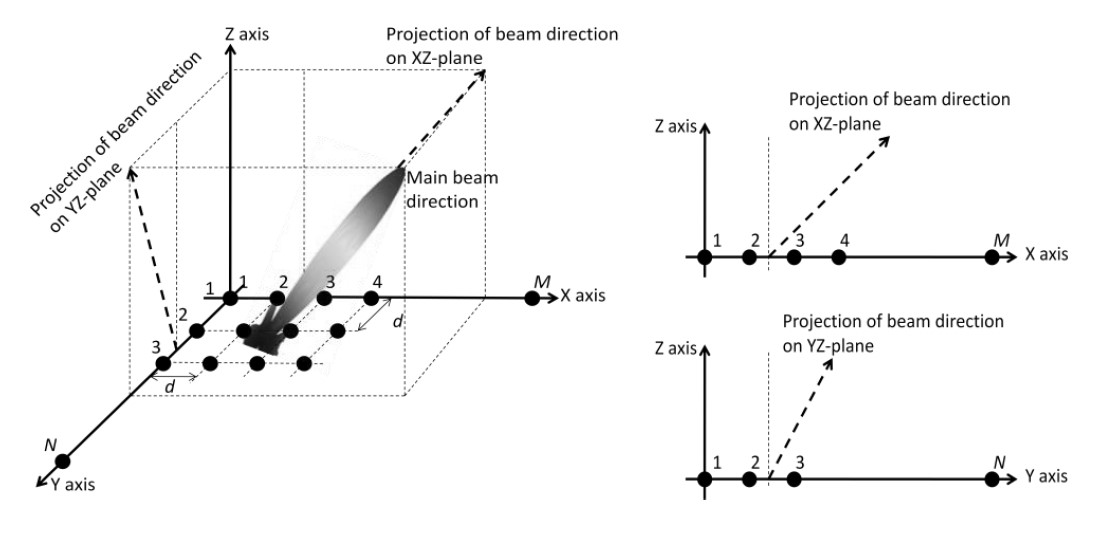
\includegraphics[width=0.9\textwidth]{images/planar_antenna}
	\caption{Schematic of a rectangular $M\times N$ planar array antenna. Source: \citep{zhuang2010ring}}
	\label{fig:planar_antenna}
\end{figure}

\section{Optical Ring Resonator}
The beamformer which will be considered in this thesis is a photonic beamformer system in which the \ac{RF} signals received by the AEs are modulated on optical carriers and tunable
optical delay lines synchronize the signals modulated on the optical carrier. The \ac{ORR} is used to implement the tunable optical delay lines. In this section, the principles of ORR will be covered including the structure, the transfer function and transfer matrix used to derive the frequency response of ORRs, and the delay properties of both single and multiple cascaded ORRs. 

\subsection{Structure of the \ac{ORR}}
A simple one input one output single stage ORR is illustrated on \figref{fig:single_stage_ORR}:

\begin{figure}[h]
	\centering
	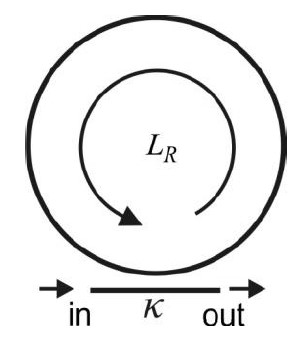
\includegraphics[width=0.2\textwidth]{images/single_stage_ORR}
	\caption{Structure of a $1 \times 1$ single-stage ORR. Source: \citep{zhuang2010ring}}
	\label{fig:single_stage_ORR}
\end{figure}

It consists of a ring-shaped waveguide and a straight waveguide. The waveguide are able to couple light between each other. The parameter $\kappa$ is the power coupling coefficient, which has the value of the range $[0\cdots 1]$, and $L_R$ is the roundtrip length of ring shaped waveguide. Another parameters are $T$ which is the roundtrip period and $\phi$ which is the extra phase-shift due to the heater on the top of the ring. 

\subsection{Mathematical Model of the \ac{ORR}}
The behavior of an optical component can be described by its transfer function (or transfer matrix when a component has multiple input/output ports), which relates the amplitude and phase of the field at input to those at output. \citet{rabus2007integrated} and \citet{zhuang2010ring} have derived the transfer function of which can be summarized as follow.

\subsubsection{Derivation of the ORR Transfer Function}

\begin{figure}[h]
	\centering
	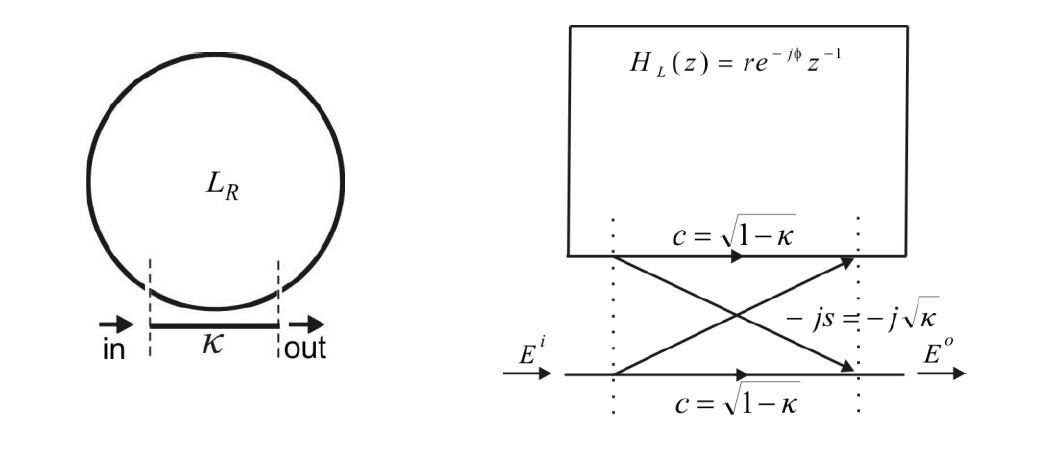
\includegraphics[width=0.8\textwidth]{images/ORR_transferfunction}
	\caption{(left) An ORR formed by a $2 \times 2$ coupler and a feedback waveguide. (right) $Z-$~transform schematic of an ORR. Source: \citep{zhuang2010ring}}
	\label{fig:ORR_transferfunction}
\end{figure}

To derive the transfer function of an ORR, one can first look at the behavior of its two basic building blocks, namely a waveguide feedback path and a $2 \time 2$ coupler, which are shown in \figref{fig:ORR_transferfunction} (left) and the $Z$-transform schematic of an ORR is given in \figref{fig:ORR_transferfunction} (right). Let the signal at the right side of the ring be $E^r$, and the one on the left side be $E^l$, then one can derive the following relations:

\begin{equation}
	\begin{aligned}
	E^r&=-j\sqrt{k}E^i+\sqrt{1-\kappa}E^l\\
	E_l&=rz^{-1}e^{j\phi}E^r \\
	&=E_l=rz^{-1}e^{j\phi}(-j\sqrt{k}E^i+\sqrt{1-\kappa}E^l)\\
	&=\frac{-j\sqrt{k}rz^{-1}e^{-j\phi}E^i}{1-r\sqrt{1-\kappa}z^{-1}e^{-j\phi}}
	\end{aligned}
\end{equation}

\begin{equation}
	\begin{aligned}
	E^o&=\sqrt{1-\kappa}E^i-j\sqrt{\kappa}E^l \\
	&=\frac{\sqrt{1-\kappa}(1-r\sqrt{1-\kappa}z^{-1}e^{-j\phi})E^i-\kappa rz^{-1}e^{-j\phi}E^i}{1-r\sqrt{1-\kappa}z^{-1}e^{-j\phi}}\\
	&=\frac{\sqrt{1-\kappa}-rz^{-1}e^{-j\phi}}{1-r\sqrt{1-\kappa}z^{-1}e^{-j\phi}}E^i
	\end{aligned}
\end{equation}

Substituting $z^{-1}=e^{-2\pi jfT}$ with $T$ the round-trip time of the ring, give the following frequency response:

\begin{equation}
	H(f)=\frac{\sqrt{1-\kappa}-re^{-2\pi jfT-j\phi}}{1-r\sqrt{1-\kappa}e^{-2\pi jfT-j\phi}}
\end{equation}

\subsubsection{Derivation of the ORR Phase Response}




%
% A Real Chapter
\chapter{Principles of Ring Resonator-Based Optical Beamforming Networks}

\section{Optical Beamforming Network Structure}


%
% A Real Chapter
\chapter{Deep Learning Neural Network for Tuning the Optical Beamforming Networks}


\section{Section 1}


%%
% Second chapter
\chapter{Some Basics}

This chapter will cover figures and math. 

\section{Figures}

Figures are constructed using the \texttt{figure} environment:
\begin{verbatim}
\begin{figure}
	\centering
	\includegraphics[options]{imagefile_location}
	\caption{Captions}
	\label{fig:dummy}
\end{figure}
\end{verbatim}

\LaTeX\ automatically decides the best placement of the Figure in your document. This will usually be at the top or bottom of the current page, or at the top of the next page. This system gives good results most of the time, but it can get confused when you have a large number of figures. The command \verb"\clearpage" creates an empty page where any `lost' figures will be printed.

You can refer to a Figure by its label: \verb"\figref{label}". See for instance \figref{fig:dummy}.

\begin{figure}
	\centering
	
\includegraphics[width=0.31415\textwidth]{STYLESTUFF/DCSC}
	\caption{The \acs{DCSC} logo. Pretty nice, eh?}
	\label{fig:dummy}
\end{figure}

\section{Math: \texorpdfstring{$e^{j \pi}=0$}{``Euler's identity''}}

I put some fancy math in the section title. Usually this generates complaints from the \texttt{hyperref} package, because the bookmarks you see on the left can only handle `regular text'. Fortunately, this problem can be solved by using a special command that inserts `regular text' whenever necessary during compilation of your thesis: \verb"\texorpdfstring{math}{text}".

For further information about math in \LaTeX, I recommend looking at the Short Math Guide found at \href{http://www.ams.org/tex/amslatex.html}{the website} of the \ac{AMS}. \index{math}

\begin{eqnarray}
% \nonumber to remove numbering (before each equation)
  1 &=& 2\\
  x &=& 5 \\
  y &=& \theta
\end{eqnarray}


\section{More About Acronyms}

After the start of a new chapter all acronyms are reset and are printed as a full acronym the first time it is used again, e.g.\ \ac{DCSC}. After the first use, only the short acronym is printed again: \ac{DCSC}.


\section{More About Nomenclature}

This is a test for nomenclature \lsymb{$A(s)$}{Answer function} \index{test}

%
%
%========================== Appendices =======================================
\appendix
%
%
% An Appendix
\chapter{The Back of the Thesis}

Appendices are found in the back. 


\section{An Appendix Section}

\subsection{An appendix subsection with C++ Listing}

\lstset{language=C++}
\lstinputlisting{test.c}

\subsection{A MATLAB listing}

\lstset{language=matlab}
\lstinputlisting{test.m}

%
% Another appendix chapter
\chapter{Yet Another Appendix}


\section{Test Section (Again?)}

Ok, all is well.


%========================== Back matter ======================================
\backmatter
%
% Bibliography
\bibliographystyle{IEEEtranN}

\bibliography{MyBib}
%
%
% Glossary
\chapter{Glossary} %
%
\printacronyms
\begin{acronym}[\hspace{0.8in}] % 0.8in is also used by the nomenclature
	\acro{3mE}[3\textlarger{m}E]{Mechanical, Maritime and Materials Engineering}%
	\acro{AMS}{American Mathematical Society}%
	\acro{DCSC}{Delft Center for Systems and Control}%
	\acro{TU}[TU D\textlarger{elft}]{Delft University of Technology}%
	\acro{OBFN}{Optical Beamforming Network}%
	\acro{ORR}{Optical Ring Resonator}%
	\acro{AE}{Antenna Element}%
	\acro{NLP}{Non-linear Programming}%
	\acro{PAA}{Phased Array Antenna}%
	\acro{RF}{Radio Frequency}%
	
\end{acronym}%
%
%
% Nomenclature
\printnomencl


%
% Index
\cleardoublepage
\printindex

\end{document}
